\dfnt{Nombres relatifs}
{On considère désormais deux types de nombres :
\begin{itemize}
    \item Les nombres positifs (+3;+1024;+3,43234)
    \item Les nombres négatifs (-4;-4321;-67,43)
\end{itemize}
On appelle l'ensemble de ces nombres les \textbf{nombres relatifs}.}


\rmq{\begin{itemize}
        \item 0 est considéré comme à la fois positif et négatifs
        \item Pour gagner du temps, le + des nombres positifs n'est souvent pas écrit.
        \item On décompose un nombre en son signe (+ ou -) et sa partie numérique (le nombre).
\end{itemize}}

\exmpl
{4; 13456789876543 et 67 sont positifs alors que -32,5467876 est négatif.
    }

\dfnt{Opposé}
{On appelle \textbf{opposé} d'un nombre, l'unique nombre ayant la même partie numérique mais ayant le signe opposé}

\rmq{
\begin{itemize}
    \item Zéro est le seul nombre ayant pour opposé lui même.
    \item L'opposé de l'opposé d'un nombre est le nombre de départ
\end{itemize}    
}

\exmpl{-4 est l'opposé de 4 et l'opposé de -4 est 4}


\dfnt{Comparer les nombres relatifs}
{
    Pour comparer deux nombres relatifs, on commence par regarder le signe :
    \begin{itemize}
        \item Pour deux nombres positifs, alors le plus grand a la plus grande partie numérique (5<14)
        \item Si il y a un nombre positif et un négatif, alors le nombre positif est plus grand (-4<2)
        \item Pour deux nombres négatifs, alors le plus grand a la plus petite partie numérique (-5<-4)
    \end{itemize}
}

\rmq{Les nombres positifs sont ceux avec lesquels on a travaillé jusqu'ici : il est donc normal que rien ne change. Pour les nombres négatifs, c'est l'inverse.}

\exmpl{-16<-7<-4<1<3<6<12}

\dfnt{Droite gradué}
{Pour placer des nombres relatifs sur une droite gradué, on commence par placer le zéro.
\\
Les nombres positifs sont placés à droite du zéro du plus petit au plus grand.
\\
Les nombres négatifs sont placés à droite du zéro du plus grand au plus petit.}

\rmq{C'est pourquoi on appelle parfois la partie numérique d'un nombre sa distance à zéro.}

\exmpl{
    \begin{figure}
        \centering
        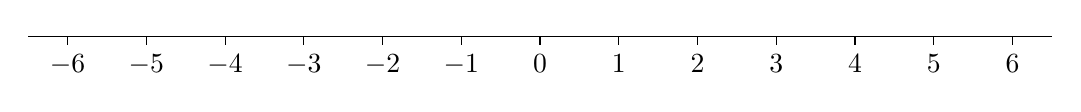
\begin{tikzpicture}
            \draw (-6.5,0) -- (6.5,0) node[midway, sloped]{};
            \foreach \x in {-6,-5,...,6}
            {
              \draw (\x,0) -- (\x,-0.1) node[below]{$\x$};
            }
        \end{tikzpicture} 
    \end{figure}
}